

\chapter{Fitness Deterioration}
\label{FitnessDeterioration}

TODO: description of the deterioration process,
not very computationally intensive,
easy to improve in subsequent runs,
interpolation accuracy is not crucial, what is most important is to
minimize the probability of finding the basins of attraction which was
previously explored,
use knowledge from clusteres;

 
\section{Sequential niching}

TODO: basic description of deterioration: 
when used, what approach,
connection with clustering algorithms,
advantages of OPTICS algorithm (improving deterioration by extracting clusters
wiht different densities, cheapness)

\subsection{Crunching functions}
When degenerating a single basin of attraction represented by a cluster of
individuals, we are looking for function with the following properties (TODO:
why):
\begin{enumerate}
  \item cheap (in multi-dimensional spaces)
  \item easily adjustable to the shape of the basin of attraction
  \item has low impact on the areas of fitness landscape which are distant from
  the cluster so that we do not introduce unnecesary noise to the fitness landscape
  in further iterations
  \item symmetric
\end{enumerate}

A class of functions which which are suitable for deterioration are so called
\textit(kernel functions) \cite{kernel}. Examples of kernels are: 
\begin{itemize}
  \item Triangular 	$K(u) = (1-|u|) \,\mathbf{1}_{\{|u|\leq1\}}$
  \item Epanechnikov 	$K(u) = \frac{3}{4}(1-u^2) \,\mathbf{1}_{\{|u|\leq1\}}$
  \item Quartic  $K(u) = \frac{15}{16}(1-u^2)^2 \,\mathbf{1}_{\{|u|\leq1\}}$
  \item Gaussian 	$K(u) = \frac{1}{\sqrt{2\pi}}e^{-\frac{1}{2}u^2}$
\end{itemize}

From mentioned function only Gaussian kernel meets all requirements (remaining
kernels are defined on some finite intervale, which makes them computationally
inefficient in high-dimensional spaces).

\section{Basic Scheme}
The basic version of our fitness crunching algorithm is as follows: \\
For each cluster generate one or more multi-dimensional Gaussian function:
\begin{equation}
 g(x)= - F_k(x_{max}) exp(\frac{-1}{2}(x-\mu)'\Sigma^{-1}(x - \mu))
\end{equation}
where $F_k$ is a fitness function in $k$th iteration of the algorithm,
$\Sigma$ is an unbiased sample covariance matrix \cite{covariance} estimated
from the cluster population:
\begin{equation}
 \Sigma = \frac{1}{n-1}\sum_{i=1}^n(x_i - \mu)(x_i - \mu)^T
\end{equation}
Fitness function in $k+1$th iteration is of the form:
\begin{equation}
 F_{k+1}=F_k + \sum_{i=1}^M g_i
\end{equation}
where M is the number of generated Gaussian functions.

Because of the fast convergence of the HGS subpopulation (and populations
generated by other algorithms) to the local minimum, clusters sometimes becomes
very dense in areas of local optimum, therefore Gaussians created for such
clusters does not approximate a basin of attraction well, speaking informaly:
Gaussian functions created for such clusters consist of high and thin peaks
which deteriorate only the area inside the cluster, not the basin of attraction
in which the cluster resides.
To overcome this issue we developed so called \textit{Covariance Matrix
Adjustment (CMA)} algorithm described in section 4.4.


\section{Adaptive Scheme}
TODO: describe in detail

detailed description of adaptive scheme deterioration

\section{Covariance Matrix Adjustment}
We use sample covariance matrix as an estimator \cite{covariance}, which is 
extremely sensitive to outliers. However we may take this property as our
advantage and incorporate it CMA algotithm. 
Having given a cluster of points the CMA algorithms works as follows:



\section{Results}

The figures below shows the result of our sequential niching algorithm for two
simple functions from $f:\mathbb{R}^2 \rightarrow \mathbb{R}$, specifically:
\begin{itemize}
  \item $f(X) = 2e^{-(x^2 + y^2)}$, where $X \in \mathbb{R}^2$
  \item $f(X) = e^{-(x^2 + y^2)}+1.4e^{-((x-1.7)^2 + (y-1.7)^2)}$, where $X \in
  \mathbb{R}^2$
\end{itemize}

\begin{figure}
  \centering
  \fbox{
    \includegraphics[scale=0.5]{deterioration1/fitnessLand.png}
  }
  \fbox{
    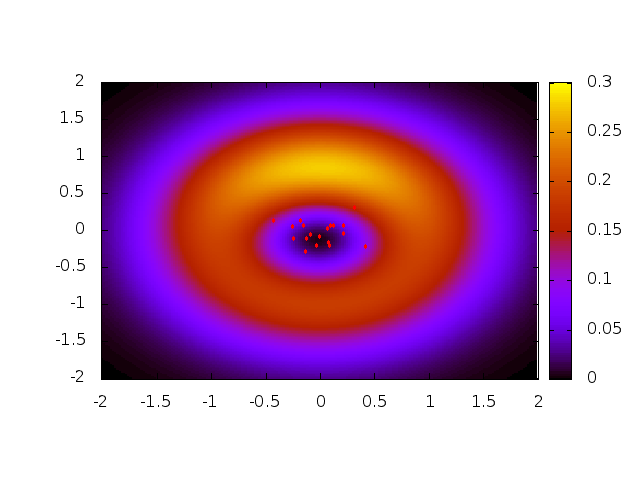
\includegraphics[scale=0.5]{deterioration1/deterioratedLandscape.png}
  }
  \caption{The result of basic deterioration scheme with CMA 
  applied to unimodal function: $f(X) = 2e^{-(x^2 +y^2)}$.
  Optics paramters: $minPts=20, \epsilon=0.4$, algorithm: SGA, iterationCount=1}
  \label{det1}
\end{figure}

\begin{figure}
  \centering
  \fbox{
    \includegraphics[scale=0.5]{deterioration3/fitnessLand.png}
  }
  \fbox{
    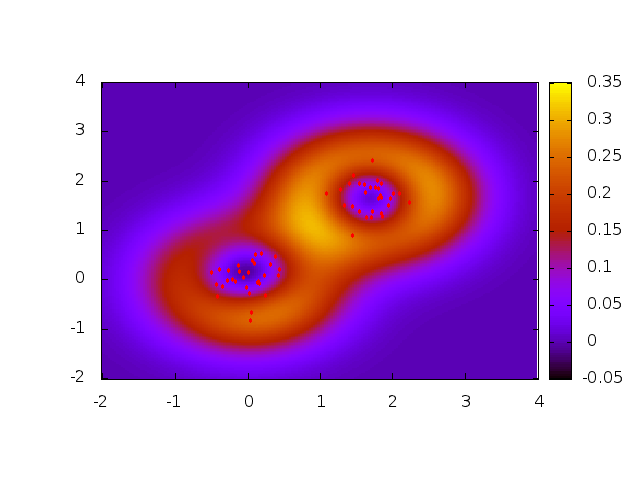
\includegraphics[scale=0.5]{deterioration3/deterioratedFitness.png}
  }
  \caption{The result of basic deterioration scheme with CMA 
  applied to bimodal function: $f(X) = e^{-(x^2 + y^2)}+1.4e^{-((x-1.7)^2 +
  (y-1.7)^2)}$. Optics paramters: $minPts=20, \epsilon=0.4$, algorithm: SGA, iterationCount=2}
  \label{det2}
\end{figure}

Figures $4.3$ and $4.4$ shows how much the algorithm benefit from using
the CMA algorithm. The plots show deterioration results applied to
functions from $4.1$ and $4.2$ without the CMA algorithm.

\begin{figure}
  \centering
  \fbox{
    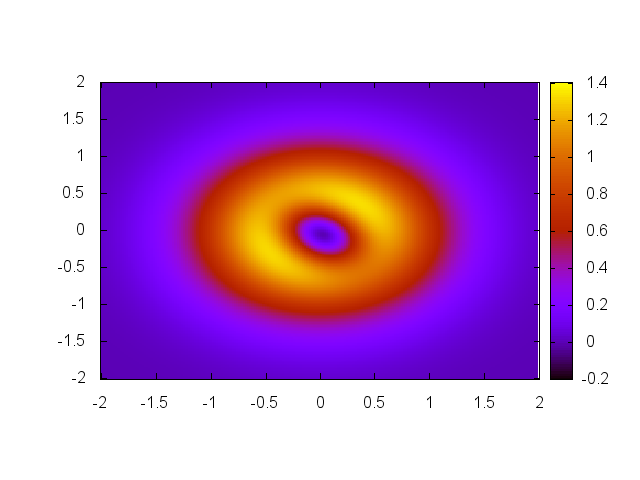
\includegraphics[scale=0.5]{deterioration4/result1_noCMA.png}
  }
  \caption{The result of basic deterioration scheme without CMA 
  applied to unimodal function from $4.1$. Optics paramters: $minPts=20,
  \epsilon=0.4$, algorithm: SGA, iterationCount=2. We may see that the 
  overall landscape decreases only by $30$ percent, while using CMA
  gives us $85$ percent of decline.}
  \label{det3}
\end{figure}

\begin{figure}
  \centering
  \fbox{
    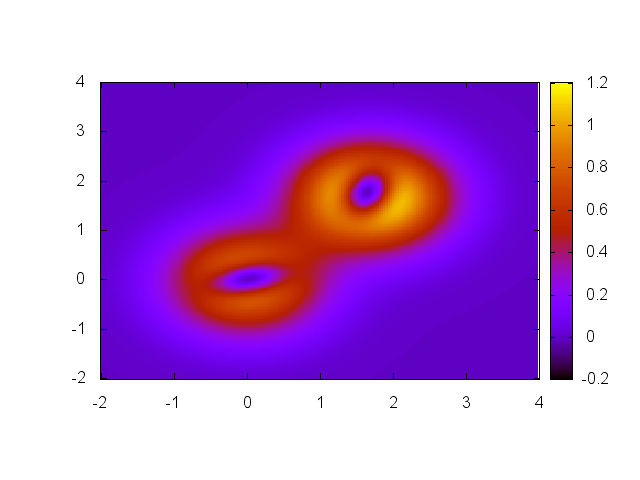
\includegraphics[scale=0.5]{deterioration4/result2_noCMA.png}
  }
  \caption{The result of basic deterioration scheme without CMA 
  applied to bimodal function from $4.2$. Optics paramters: $minPts=20,
  \epsilon=0.4$, algorithm: SGA, iterationCount=2. We see $25$ percent
  of deterioration, while CMA gives us $78$ percent when applied to the same
  case.}
  \label{det3}
\end{figure}

